\documentclass[12pt,a4paper]{report}

\usepackage[left=2cm, right=2cm, top=5cm]{geometry}
\usepackage{enumitem}
\usepackage{fontspec}
\usepackage{tikz}
\usepackage{amsmath}

\usepackage{algpseudocode}
\algblockdefx[Initially]{Initially}{EndInitially}{\textbf{initially do}}{\textbf{end initially}}
\algblockdefx[Upon]{Upon}{EndUpon}[1]{\textbf{upon #1}}{\textbf{end upon}}
\algblockdefx[AsSoon]{AsSoon}{EndAsSoon}[1]{\textbf{upon #1}}{\textbf{end as soon}}

\usetikzlibrary{graphs, shapes, graphdrawing}
\usegdlibrary{layered, force}

\begin{document}

	\newcommand{\upon}[1]{\textbf{Upon} #1 \textbf{do}}

	\begin{titlepage}
		\centering
		{\scshape\LARGE Universidad Nacional Autónoma de México \par}
		\vspace{1cm}
		{\scshape\Large Computación Distribuida\par}
		\vspace{1.5cm}
		{\huge\bfseries Tarea 6\par}
		\vspace{.5cm}
		{\Large\itshape Edgar Quiroz Castañeda \par}
	    \vspace{.5cm}
		{\Large\itshape Jerónimo Almeida Rodríguez \par}
		\vfill
		 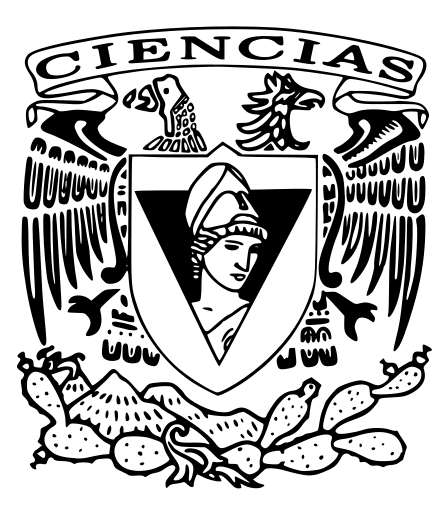
\includegraphics[width=0.5\textwidth]{escudo_f-ciencias.png}
		\vfill

		{\large Jueves 1 de octubre del 2018 \par}
	\end{titlepage}

	\pagebreak
	\setlength{\voffset}{-0.75in}
	\setlength{\headsep}{5pt}

	\begin{enumerate}
		\item {
			Sea $G = (V, E)$ una gráfica. Diseña un algoritmo $BFS$ basado en correr
			$|V|$ instancias del algoritmo $PIF$ cuya complejidad ser
			$O(|E|+|V|\cdot Diam(G))$ en mensajes y $O(Diam(G)^2)$ en tiempo.

			\begin{algorithmic}[1]
				\Require $p_{id}, root$
				\Statex
				\Initially
					\State $children \gets \emptyset$
					\State $nonChildren \gets \emptyset$
					\State $currentBound \gets 0$
					\If{$p_{id} = root$}
						\State $distance \gets 0$
						\State $parent \gets p_{id}$
						\State $currentBound \gets 1$
						\State send $(distance, 1)$ to $neighbors\setminus \{p\}$
					\Else
						\State $parent \gets \bot$
						\State $distance \gets \infty$
					\EndIf
				\EndInitially
				\Statex
				\Upon{receiving $(distance_p, bound)$ from $p$}
					\If{$distance_p + 1 < distance$}
						\State $distance \gets distance_p + 1$
						\State $parent \gets p$
						\If{$bound - 1 < distance$}
							\State send $(distance, bound)$ to $children$
						\ElsIf{$bound - 1 = distance$}
							\State send $(distance, bound)$ to $neighbors\setminus \{p\}$
						\Else
							\State send $(ack, bound)$ to $parent$
						\EndIf
					\Else
						\State send $nack$ to $p$
					\EndIf
				\EndUpon
				\Statex
				\Upon{receiving $(ack, bound)$ from $p$}
					\If{$p_{id} = root$}

					\Else
					\EndIf
					\State $children \gets children \cup \{p\}$
				\EndUpon
				\Statex
				\Upon{receiving $nack$ from $p$}
					\State $nonChildren \gets nonChildren \cup \{p\}$
				\EndUpon
				\Statex
			\end{algorithmic}
		}
		\item {
			Explicar por qué el algorítmo Awerbuch $DFS$ tiene complejidad de tiempo
			$O(V)$ ($4|V|-2$) y en mensajes $O(E)$ ($4|E|$). Presentar un ejemplo
			de ejecución en la siguiente gráfica

			\begin{center}
				\begin{tikzpicture}[node distance = 3cm]
					\begin{scope}[every node/.style = {circle, draw}]
						\node (p1) {$p_1$};
						\node (p2) [above right of = p1] {$p_2$};
						\node (p3) [right of = p2] {$p_3$};
						\node (p4) [below right of = p3] {$p_4$};
						\node (p5) [left of = p4] {$p_4$};
						\node (p6) [below right of = p1] {$p_6$};
					\end{scope}

					\path[-] (p1) edge (p2);
					\path[-] (p1) edge (p5);
					\path[-] (p1) edge (p6);

					\path[-] (p2) edge (p3);
					\path[-] (p2) edge (p4);

					\path[-] (p3) edge (p4);

					\path[-] (p4) edge (p5);
					\path[-] (p4) edge (p6);

					\path[-] (p5) edge (p6);
				\end{tikzpicture}
			\end{center}
		}
		\item {
			Ver el video y mediante una lista de puntos explicar las ideas que se
			exponon. Cada punto no debe tener más de un par de líneas.
			The Physics and Philosophy of Time - with Carlo Rovelli https://youtu.be/-6rWqJhDv7M
		}
	\end{enumerate}
\end{document}
